\section{Results and Discussion}
This section describes the results obtained from the three main sections of this project. 
\subsection{Final Design}
The complete design in exploded view is shown in figure \ref{fig:unit_exploded_view}.
\begin{figure}[H]
    \centering
    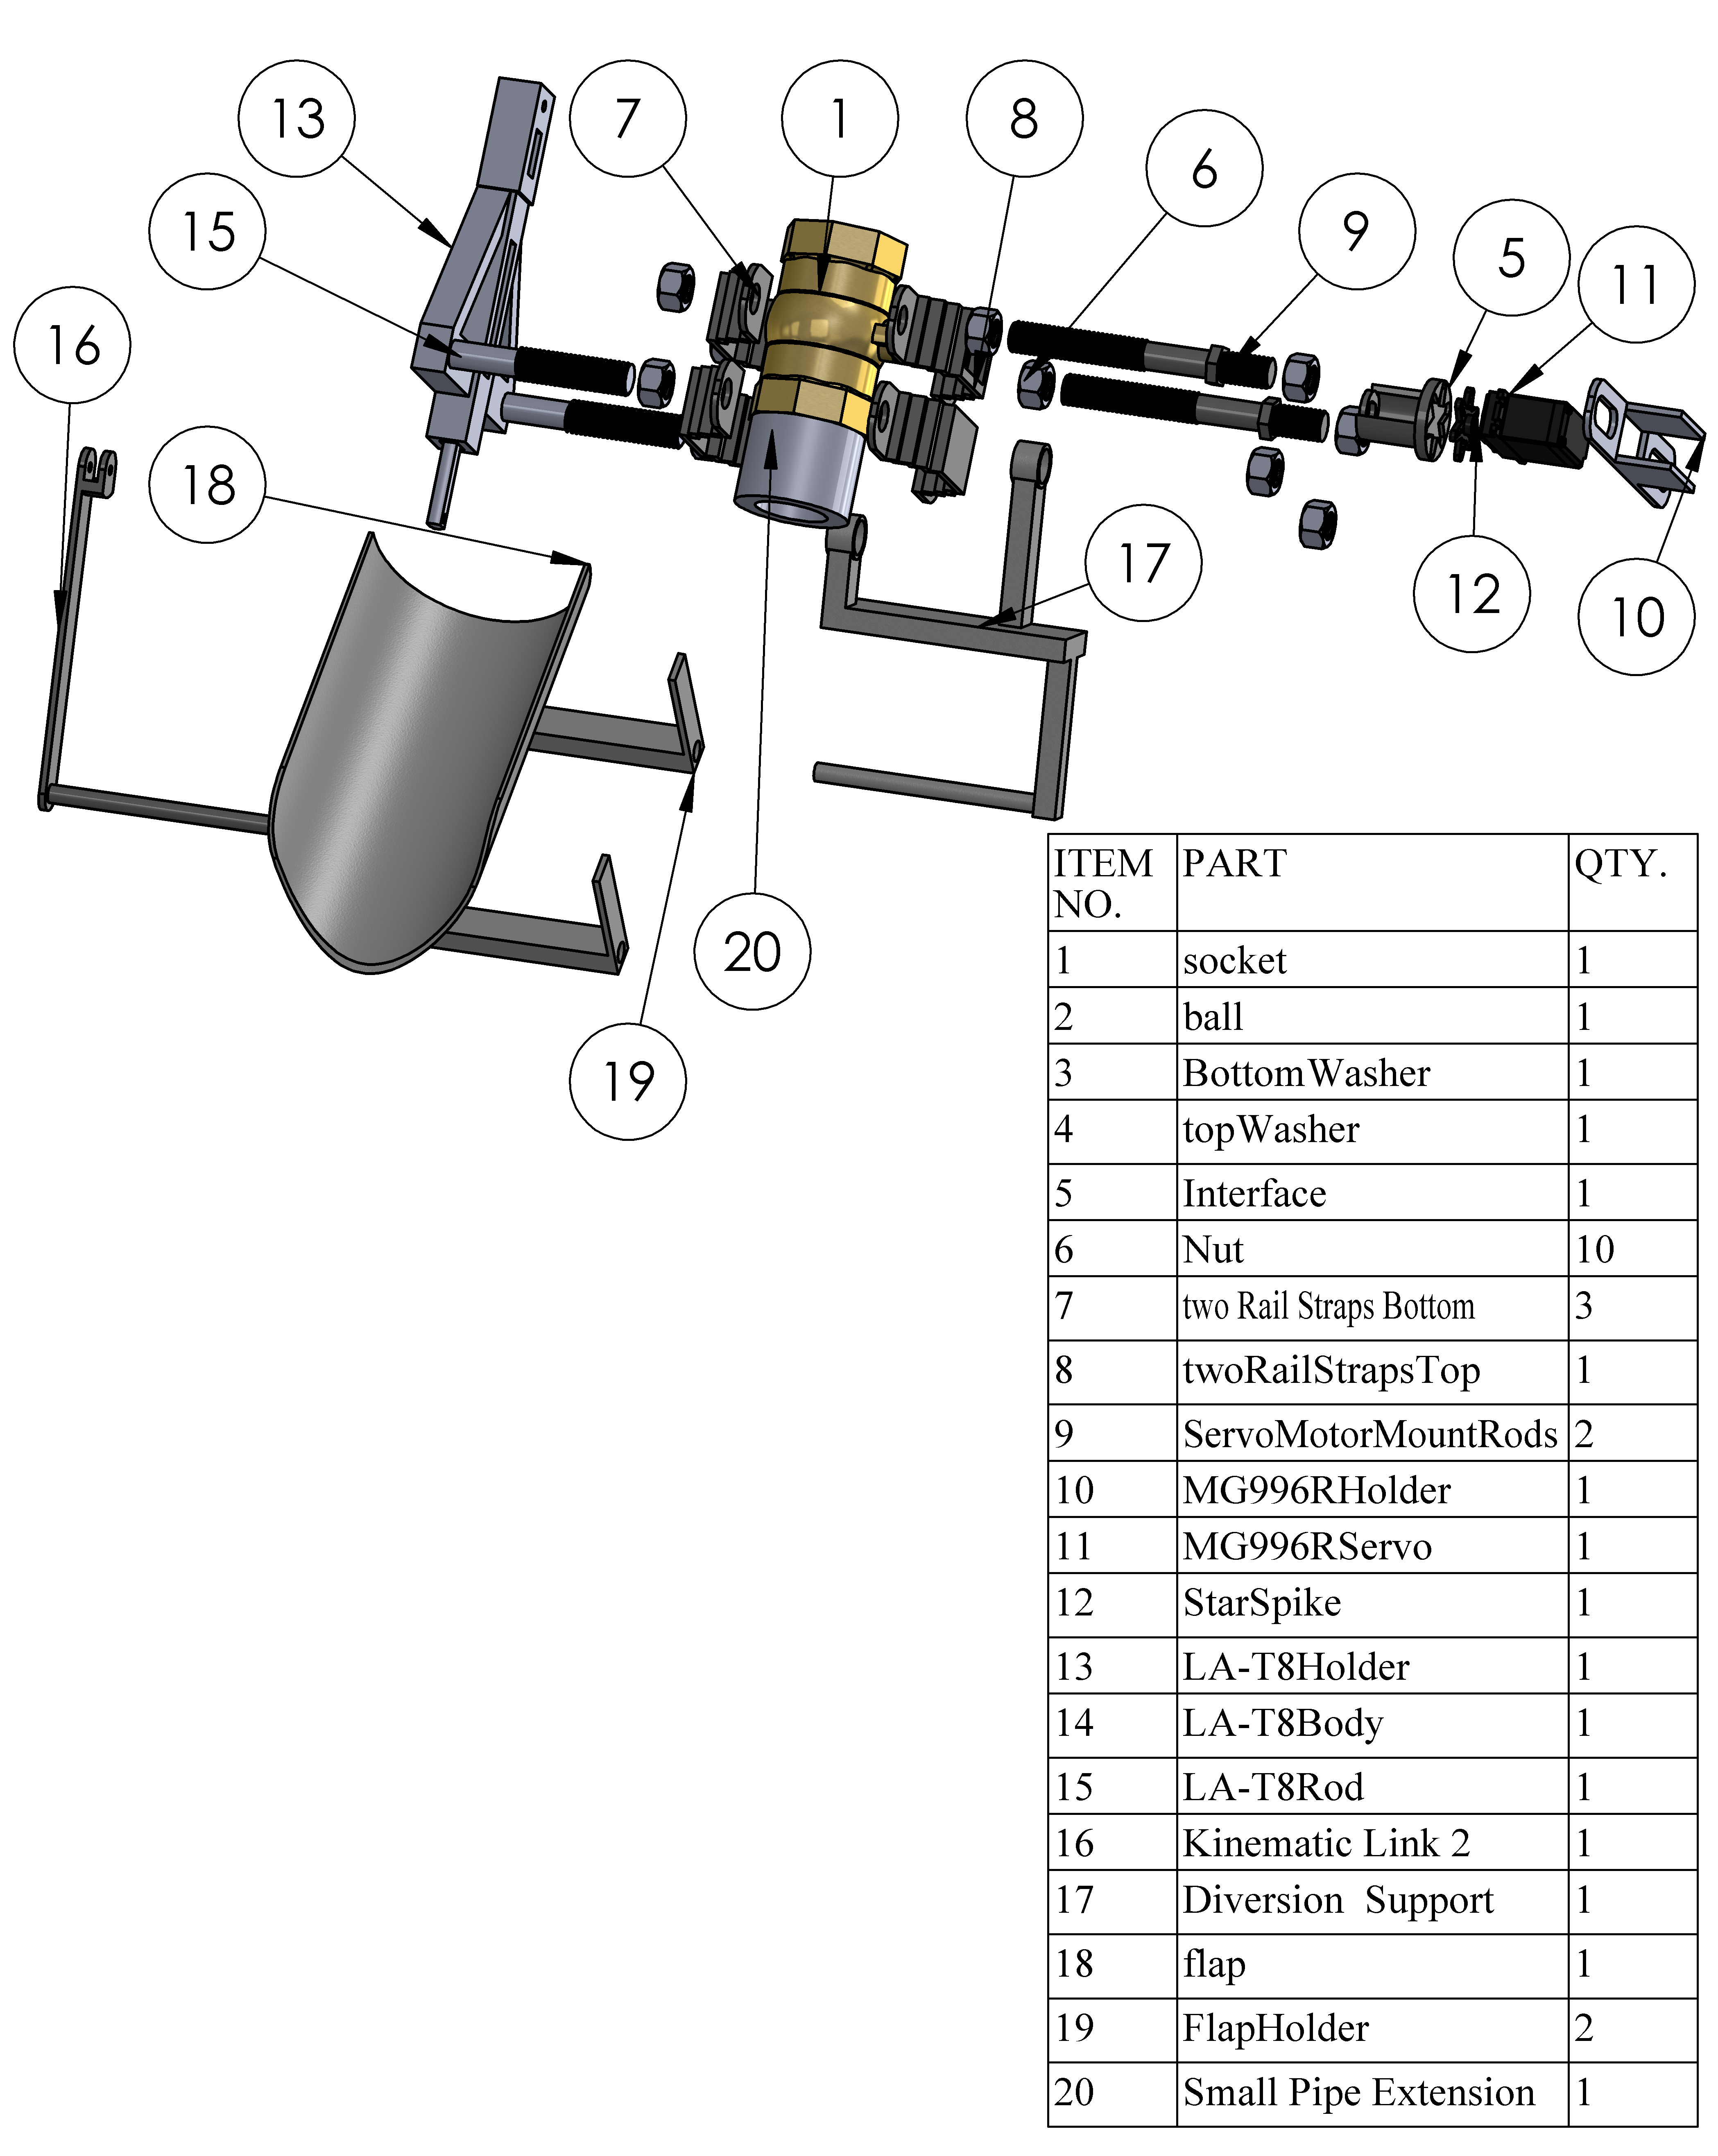
\includegraphics[height=.7\textheight]{Figures/DischargeFlowControlAssemblyExploded.PNG}
    \caption{Unit Exploded view}
    \label{fig:unit_exploded_view}
\end{figure}
\subsection{The Discharge Flow Control unit}
The objective of this unit was to design and fabricate an automated flow control mechanism that can operate the ball valve in steps of less than 1 degree and a flow diverter mechanism that can divert the flow in a second. 
\par
Figure \ref{fig:Setting the number of steps from the user interface} shows the virtual arc dial labelled 'Valve' that is used for opening and closing the ball valve. The dial has been programmed to operate the servo motor in steps of 1 degree.
\begin{figure}[H]
\centering
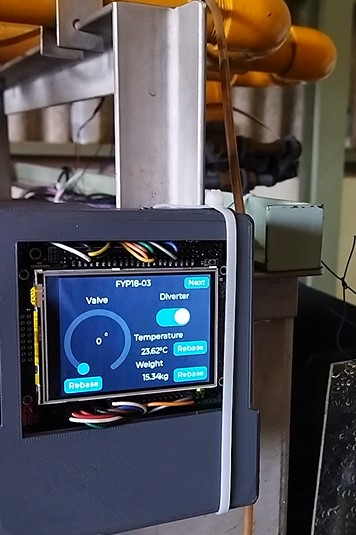
\includegraphics{Figures/flow_cotrol_control.jpg}
\caption{Controls for the flow control}
\label{fig:Setting the number of steps from the user interface}
\end{figure}
The protrusion on the ball valve, marking the closed position of the valve lever was used as a datum for testing and calibration. A full rotation from one face of the protrusion to the other about the center of the ball valve is equal to a 90-degree rotation. The selected servo motor covers this in just only a 76-degree rotation. This is a clear indication that the selected servo motor can turn in steps of less than 1 degree.
\par
The LAT8 linear actuator used for flow diversion could divert the flow in between 1 second and 1.5 seconds depending on the pressure set in the main pump. Pressure equivalent to a barometric height of 390 mm across the venturi was found to be ideal for diversion in 1.2 seconds.
\par
Figure \ref{fig:Discharge Flow Control Unit} shows the assembly of the fabricated unit. 
\begin{figure}[H]
\centering
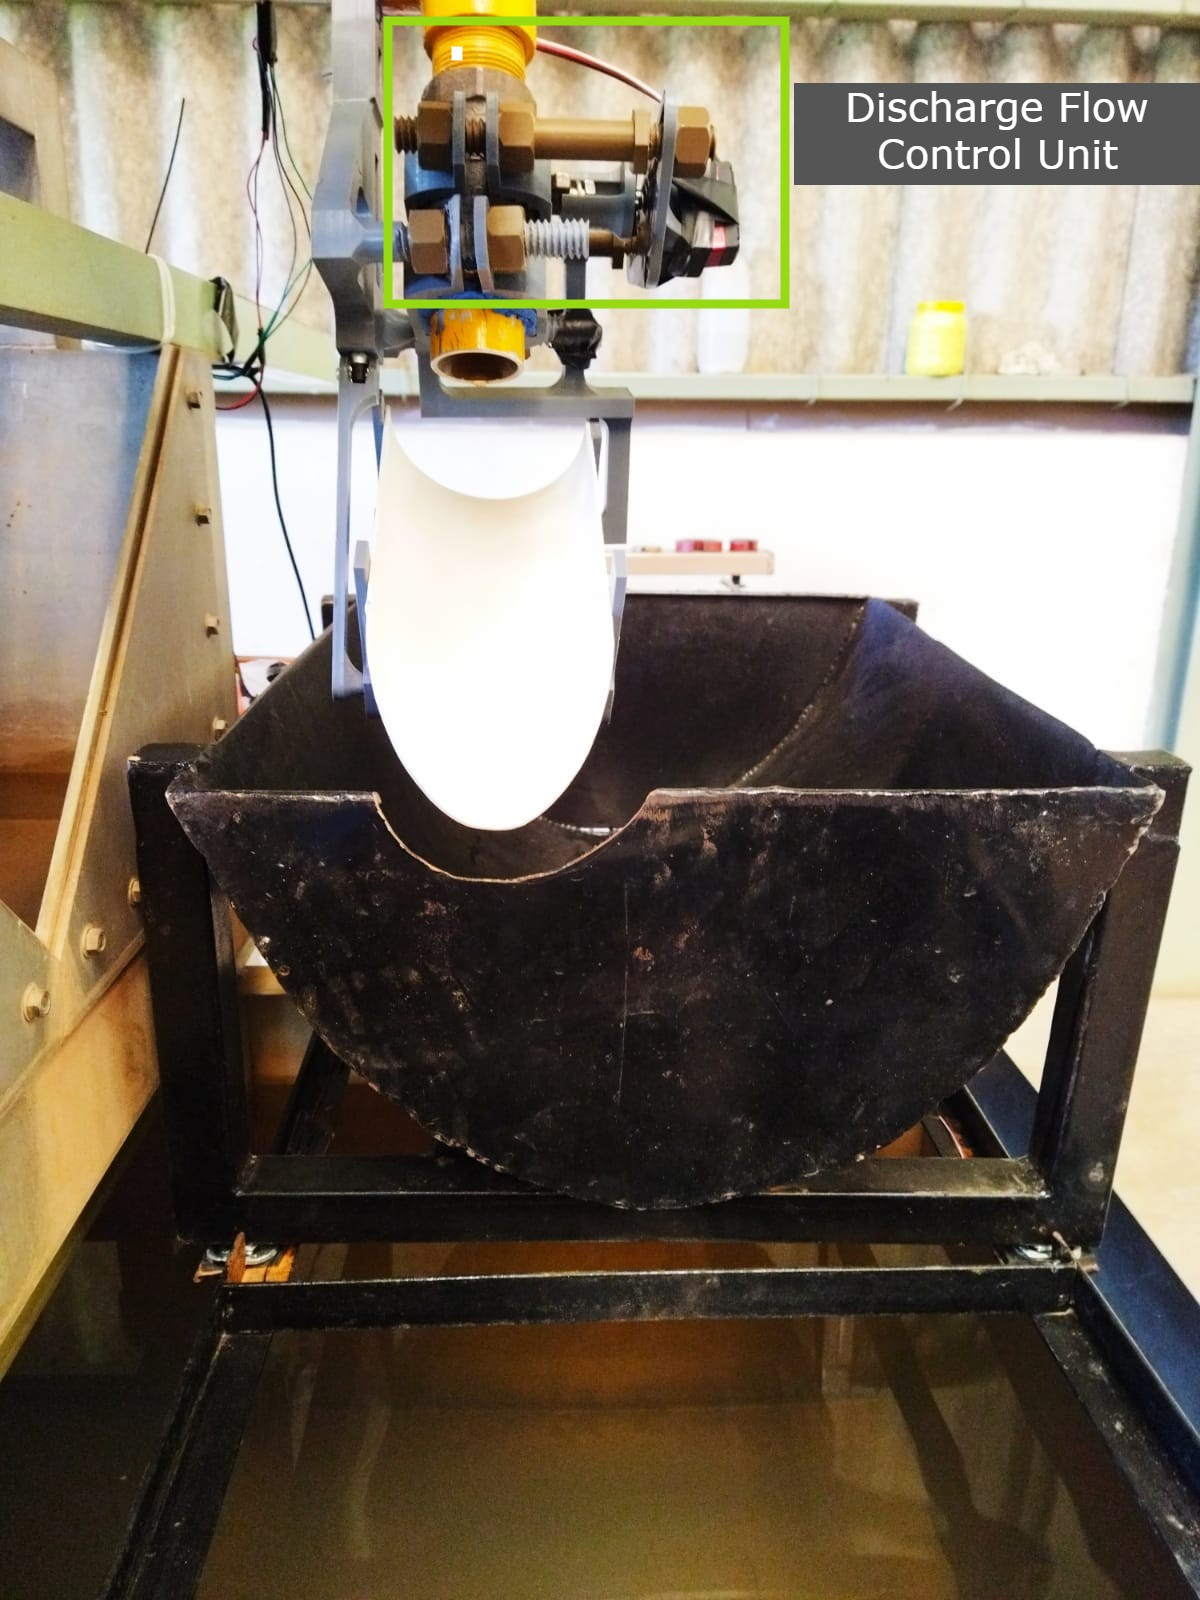
\includegraphics[width=.55\textwidth]{Figures/flow control Results.jpg}
\caption{Discharge Flow Control Unit}
\label{fig:Discharge Flow Control Unit}
\end{figure}
\subsection{The discharge handling unit}
The objective was to automate weight and temperature measurements, and re-design the discharge collection tank such that it can discharge in the least time possible. 
\par 
A DS18B20 temperature probe and four load cells were used for measuring temperature, and the weight of the collected discharge after every 200 ms. These values are continuously displayed on the interface. 
\par
The tank could also collect 25 kg of discharge, and is fitted with a $1 \frac{1}{2} inch$ ball valve at the bottom that can discharge a full tank in 12.73 seconds.
\par
Figure \ref{fig: Discharge Handling Unit} below, shows the assembly of the fabricated unit. 
\begin{figure}[H]
\centering
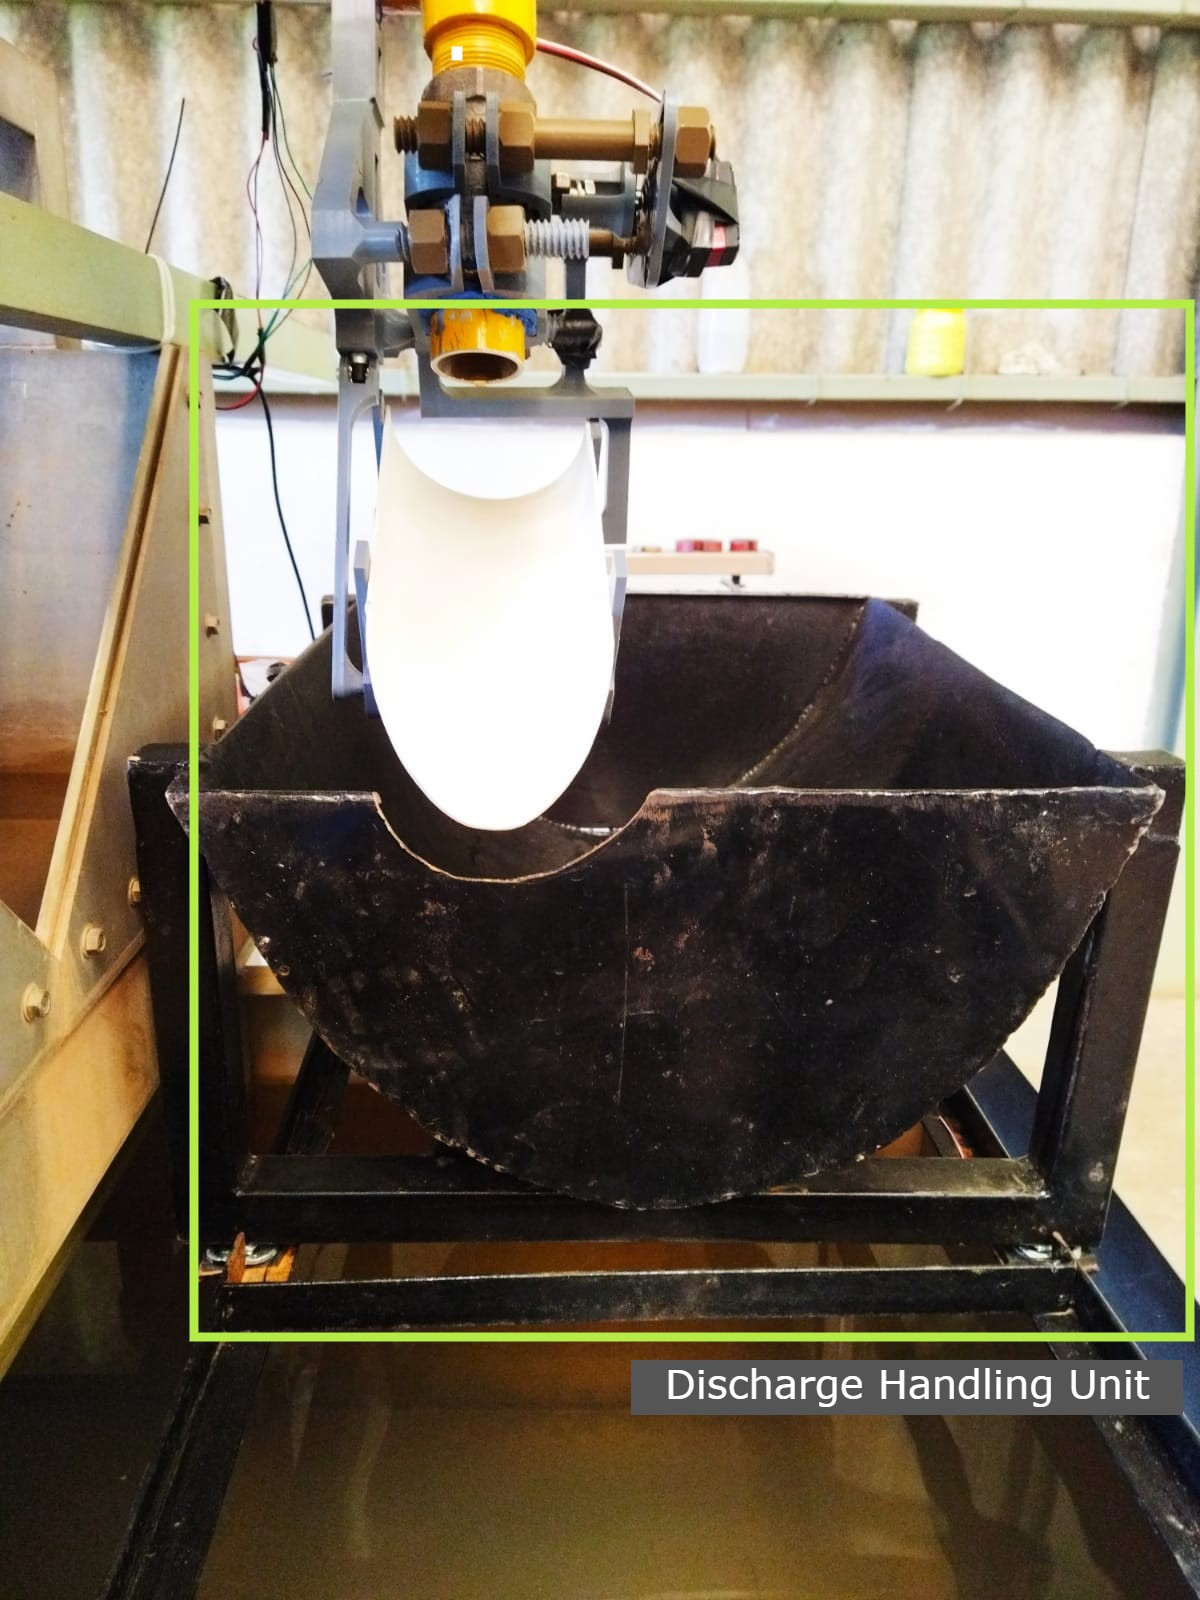
\includegraphics[height=.5\textheight]{Figures/discharge handling results.jpg}
\caption{Discharge Handling Unit}
\label{fig: Discharge Handling Unit}
\end{figure}

\subsection{Electrical and Electronics Unit}
Figure \ref{fig: Electrical Assembly} and \ref{fig: User Interface Mounted} show the electrical and electronic components developed on a proto-board including the components for the servo motor control, an LA-T8 electromagnet linear actuator control, an HX711, and a DS18B20 temperature probe. 
\begin{figure}[H]
\centering
\includegraphics[width=.7\textwidth]{Figures/proto_board_assembled.jpg}
\caption{Electrical Assembly}
\label{fig: Electrical Assembly}
\end{figure}
        
\begin{figure}[H]
\centering
\includegraphics[width=.7\textwidth]{Figures/proto_board_front.jpg}
\caption{User Interface Mounted}
\label{fig: User Interface Mounted}
\end{figure}
\subsection{Final Assembly}
\par 
Figure \ref{fig: Finally Assembly} below shows the final assembly inclusive of the discharge flow control unit, discharge handling unit, and the interface and control unit. The unit is designed and fabricated as a plug-and-play, in that it is not permanently fixed onto the machine but can be removed to allow for other experiments to be conducted.
\begin{figure}[H]
            \centering
            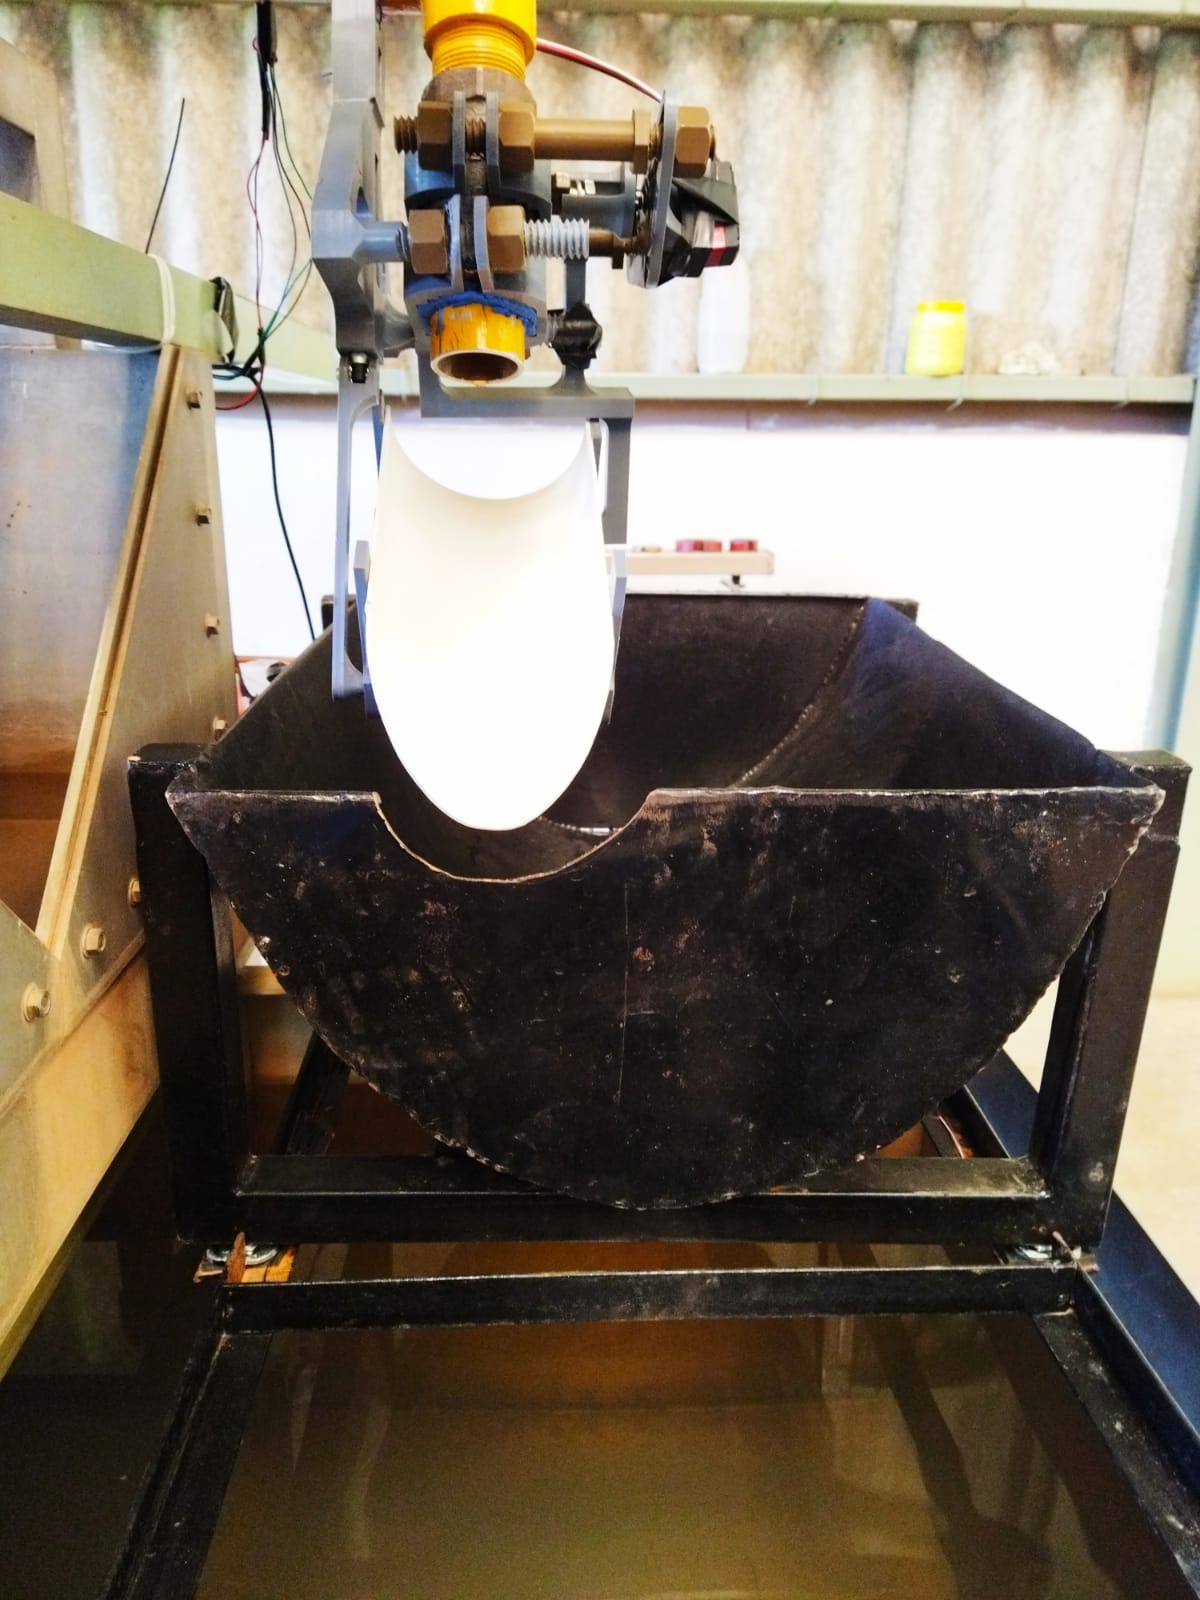
\includegraphics[width=.7\textwidth]{Figures/FinalAssembly.jpeg}
            \caption{Finally Assembly}
            \label{fig: Finally Assembly}
        \end{figure}

\subsection{Experiments Conducted}

The coefficient of discharge experiments was conducted using the system. The objective was to determine the coefficient of discharge from the system and compare it with the one obtained from manually conducting the experiment. This was so as to determine whether the system reduced the human error that resulted from the manual operation of the test rig. 
\par
During the experiment, four runs were conducted in total. One involved manual operation while three were done with the automated system.  With the system in place, it first reduced the number of operators from three to two. Secondly, when conducting the experiment, the user is required to only set the number of steps (runs) to perform the experiment and the maximum time interval. The system then auto-calibrates itself to determine the time allocation for each run. The results from each run are recorded via the necessary components and the values sent to be recorded under time, temperature, and weight. 
\subsubsection{Experiment 1}
Table \ref{tab:manual_exp} below shows the results obtained from the manual operation to determine the coefficient of discharge of the venturi.

% Please add the following required packages to your document preamble:
% \usepackage{graphicx}
\begin{table}[H]
\centering
\caption{Manual Experiment}
\label{tab:manual_exp}
\resizebox{\textwidth}{!}{%
\begin{tabular}{|l|l|l|l|l|l|l|l|l|}
\hline
\textbf{Step} & \textbf{Height 1} & \textbf{Height 2} & \textbf{Head} & \textbf{Weight 1} & \textbf{Weight 2} & \textbf{Weight} & \textbf{Temperature} & \textbf{Time} \\ \hline
0  & 0   & 0   & 0   & 0     & 0     & 0                & 0  & 0     \\ \hline
1  & 665 & 657 & 8   & 22    & 27.4  & 5.4              & 21 & 50.51 \\ \hline
2  & 657 & 642 & 15  & 27.4  & 36.1  & 8.7              & 21 & 42.56 \\ \hline
3  & 647 & 613 & 34  & 36.1  & 40.9  & 4.8              & 21 & 30.3  \\ \hline
4  & 623 & 514 & 109 & 40.9  & 58.1  & 17.2             & 22 & 21.74 \\ \hline
5  & 594 & 428 & 166 & 58.1  & 67.7  & 9.6              & 22 & 18.44 \\ \hline
6  & 562 & 317 & 245 & 67.7  & 81.1  & 13.4             & 22 & 15.39 \\ \hline
7  & 548 & 282 & 266 & 81.1  & 93.7  & 12.6             & 22 & 12.53 \\ \hline
8  & 522 & 212 & 310 & 93.7  & 103.6 & 9.89999999999999 & 22 & 8.05  \\ \hline
9  & 500 & 153 & 347 & 106.6 & 111.5 & 4.90000000000001 & 22 & 5.13  \\ \hline
10 & 474 & 85  & 389 & 111.5 & 115.3 & 3.8              & 22 & 3.6   \\ \hline
\end{tabular}%
}
\end{table}
From table \ref{tab:manual_exp}, a graph of the actual flow rate $(Q_\text{act})$ versus the square root of the differential $\left(h_1-h_2\right)^{1 / 2}$ head was plotted as shown in Figure \ref{fig: Manual Experiment}. The coefficient of discharge $C_d$ was found to be 0.747773.
\begin{figure}[H]
            \centering
        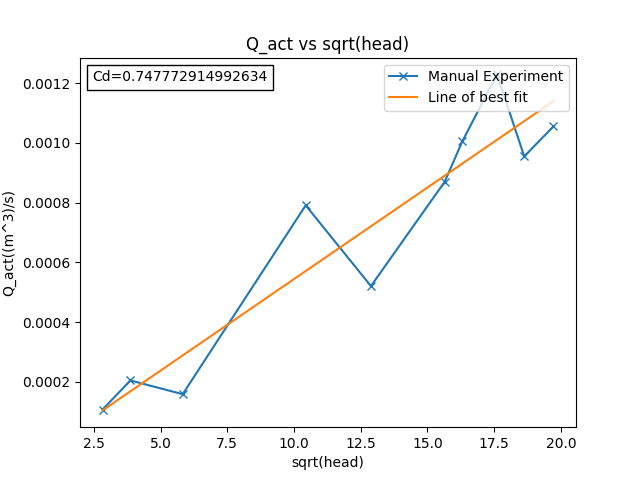
\includegraphics[width=.85\textwidth]{Figures/Manual_Exp.png}
            \caption{Manual Experiment}
            \label{fig: Manual Experiment}
        \end{figure}
\subsubsection{Experiment 1}
\par
The results from the second experiment are tabulated in table \ref{tab:experiment_1} below.
% Please add the following required packages to your document preamble:
% \usepackage{graphicx}
\begin{table}[H]
\centering
\caption{Experiment 1}
\label{tab:experiment_1}
\resizebox{\textwidth}{!}{%
\begin{tabular}{|l|l|l|l|l|l|l|l|l|}
\hline
\textbf{Step 1} &
  \textbf{Height 1} &
  \textbf{Height 2} &
  \textbf{Head} &
  \textbf{Weight 1} &
  \textbf{Weight 2} &
  \textbf{Weight} &
  \textbf{Temperature(deg. C)} &
  \textbf{Time} \\ \hline
0  & 390 & 390 & 0   & 5.61 & 5.61  & 0     & 24.5  &    \\ \hline
1  & 390 & 375 & 15  & 5.61 & 12.2  & 6.59  & 23.62 & 38 \\ \hline
2  & 365 & 345 & 20  & 5.14 & 12.56 & 7.42  & 23.38 & 34 \\ \hline
3  & 315 & 280 & 35  & 5.36 & 15.94 & 10.58 & 23.44 & 30 \\ \hline
4  & 287 & 237 & 50  & 5.76 & 18.45 & 12.69 & 23.5  & 26 \\ \hline
5  & 244 & 188 & 56  & 5.79 & 19.05 & 13.26 & 23.5  & 23 \\ \hline
6  & 205 & 133 & 72  & 5.79 & 18.7  & 12.91 & 23.56 & 19 \\ \hline
7  & 177 & 90  & 87  & 5.75 & 17.64 & 11.89 & 23.5  & 15 \\ \hline
8  & 150 & 59  & 91  & 5.75 & 16    & 10.25 & 23.62 & 12 \\ \hline
9  & 135 & 29  & 106 & 5.74 & 13.6  & 7.86  & 23.56 & 8  \\ \hline
10 & 116 & 3   & 113 & 5.67 & 11    & 5.33  & 23.56 & 4  \\ \hline
\end{tabular}%
}
\end{table}
\par
The coefficient of discharge $C_d$ from the graph of the actual flow rate $(Q_\text{act})$ versus the square root of was found to be as shown in figure \ref{fig: Experiment1}. The $C_d$ from experiment 2 was however way below the actual $C_d$ with a percentage error of approximately 15 percent.
\begin{figure}[H]
            \centering
        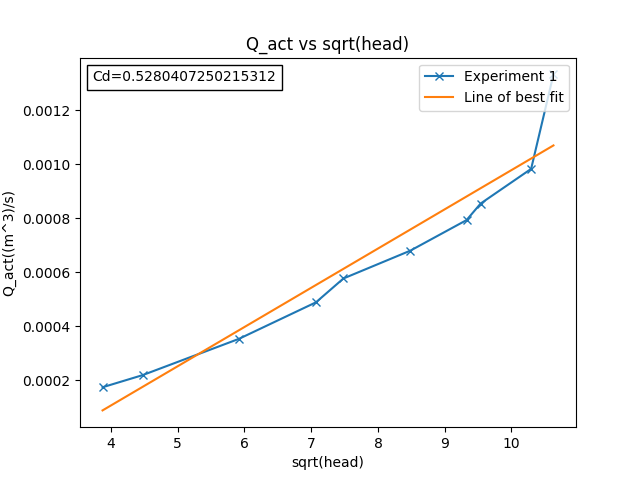
\includegraphics[width=.85\textwidth]{Figures/Experiment1.png}
            \caption{Experiment1}
            \label{fig: Experiment1}
        \end{figure}
% Please add the following required packages to your document preamble:
% \usepackage{graphicx}
\subsubsection{Experiment 2}
The results from the third experiment are shown in table \ref{tab:experiment_2}
\begin{table}[H]
\centering
\caption{Experiment 2}
\label{tab:experiment_2}
\resizebox{\textwidth}{!}{%
\begin{tabular}{|l|l|l|l|l|l|l|l|l|}
\hline
\textbf{Step} &
  \textbf{Height 1} &
  \textbf{Height 2} &
  \textbf{Head} &
  \textbf{Weight 1} &
  \textbf{Weight 2} &
  \textbf{Weight} &
  \textbf{Temperature(deg. C)} &
  \textbf{Time} \\ \hline
0 & 410 & 410 & 0   & 6.13 & 6.13  & 0     & 22.5  &    \\ \hline
1 & 375 & 360 & 15  & 6.13 & 14.34 & 8.21  & 22.94 & 38 \\ \hline
2 & 359 & 342 & 17  & 6.01 & 15.9  & 9.89  & 23.06 & 34 \\ \hline
3 & 330 & 295 & 35  & 6.11 & 18.85 & 12.74 & 23.12 & 30 \\ \hline
4 & 295 & 243 & 52  & 6.11 & 20.55 & 14.44 & 23.19 & 27 \\ \hline
5 & 256 & 185 & 71  & 6.11 & 21.25 & 15.14 & 23.19 & 23 \\ \hline
6 & 214 & 119 & 95  & 6.2  & 21.05 & 14.85 & 23.25 & 19 \\ \hline
7 & 192 & 56  & 136 & 6.13 & 21.25 & 15.12 & 23.25 & 15 \\ \hline
\end{tabular}%
}
\end{table}
Figure \ref{fig: Experiment2} depicts the coefficient of discharge (0.76198) from the second round. 
\begin{figure}[H]
            \centering
        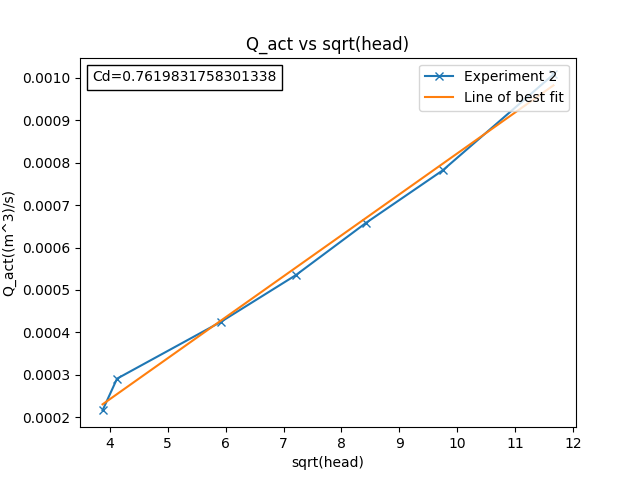
\includegraphics[width=.85\textwidth]{Figures/Experiment2.png}
            \caption{Experiment2}
            \label{fig: Experiment2}
        \end{figure}
\subsubsection{Experimnet 3}
\par
The results from the third run are illustrated in table \ref{tab:experiment_3}.
% Please add the following required packages to your document preamble:
% \usepackage{graphicx}
\begin{table}[H]
\centering
\caption{Experiment 3}
\label{tab:experiment_3}
\resizebox{\textwidth}{!}{%
\begin{tabular}{|l|l|l|l|l|l|l|l|l|}
\hline
\textbf{Step} &
  \textbf{Height 1} &
  \textbf{Height 2} &
  \textbf{Head} &
  \textbf{Weight 1 (kg)} &
  \textbf{Weight 2 (kg)} &
  \textbf{Weight} &
  \textbf{Temp (degrees)} &
  \textbf{Time} \\ \hline
0 & 327 & 327 & 0  & 6.28 & 6.28  & 0     & 21.81 &    \\ \hline
1 & 275 & 265 & 10 & 6.28 & 16    & 9.72  & 21.88 & 48 \\ \hline
2 & 250 & 231 & 19 & 5.28 & 18.23 & 12.95 & 22    & 43 \\ \hline
3 & 205 & 165 & 40 & 5.39 & 21.72 & 16.33 & 22.12 & 38 \\ \hline
4 & 157 & 105 & 52 & 5.39 & 23.1  & 17.71 & 22.19 & 33 \\ \hline
5 & 121 & 56  & 65 & 5.41 & 22.95 & 17.54 & 22.19 & 28 \\ \hline
6 & 88  & 13  & 75 & 5.4  & 21.67 & 16.27 & 22.25 & 23 \\ \hline
\end{tabular}%
}
\end{table}
\par
The graphical illustration of a graph of the actual flow rate $(Q_\text{act})$ versus the square root resulted in the final coefficient of discharge of 0.82175. Compared to the results from the manual experiment, there was a 8.213 \% percent reduction in the overall error. 
\begin{figure}[H]
            \centering
        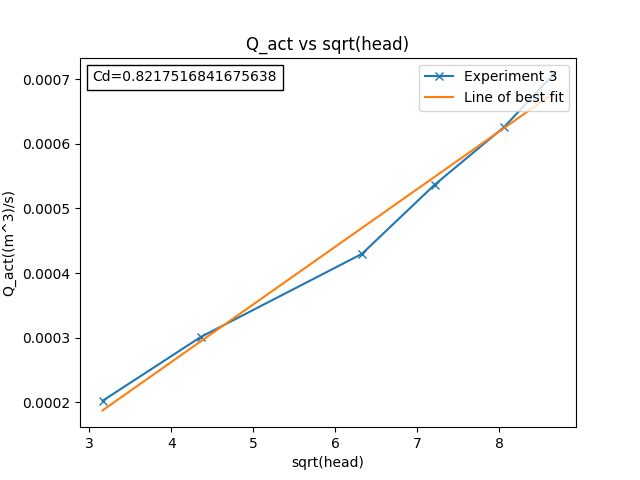
\includegraphics[width=.85\textwidth]{Figures/Experiment3.png}
            \caption{Experiment3}
            \label{fig: Experiment3}
        \end{figure}
\par
The system reduced the overall human error margin that arises from the manual operation of the experiment by approximately 10 percent as depicted from the values obtained in the second and final run of the experiment. The calculations were based on the average coefficient of discharge of the venturi, 0.985. The first automatic run was however not as successful as anticipated. This was because of the very high-pressure discharge from the main pipeline that strained the LA-T8 electromagnet linear actuator leading to delays in discharge diversion and thus incorrect readings. The pressure was however adjusted to the required level.